% !TEX encoding = UTF-8 Unicode
\chapter{Les r\'esultats compl\'ementaires des \mt utilisent }

\label{annexe}
\section{Exploration des résultats d'analyse sous-séquence de la méthode Causalité de Granger uni-variable et multivariable}

Plus précisément, nous allons mettre en place les diagrammes montrant la fréquence des provinces importantes pour chaque période. Les figures \ref {expl_1}, \ref {expl_2}, \ref {expl_3}, \ref {expl_4}, \ref {expl_5}, \ref {expl_6}, \ref {expl_7} illustrent le diagramme de fréquence des provinces importantes par la fréquence avec la longueur de la période est égale à 6. Les provinces ayant une position basse sur l’axe des Y représentent une forte corrélation avec le facteur climatique tout au long de leur période. 

Les figures \ref {expl_8}, \ref {expl_9}, \ref {expl_10}, \ref {expl_11}, \ref {expl_12}, \ref {expl_13}, \ref {expl_14} montrent le diagramme de fréquence des provinces importantes classées par latitude de chaque province avec la durée de la période est égale à 6. Nous pouvons voir que quand une épidémie de dengue sur une province montre que la relation avec le facteur climatique dans une période continue à montrer sa relation dans les périodes plus récentes.


\begin{figure}[h]
\begin{center}
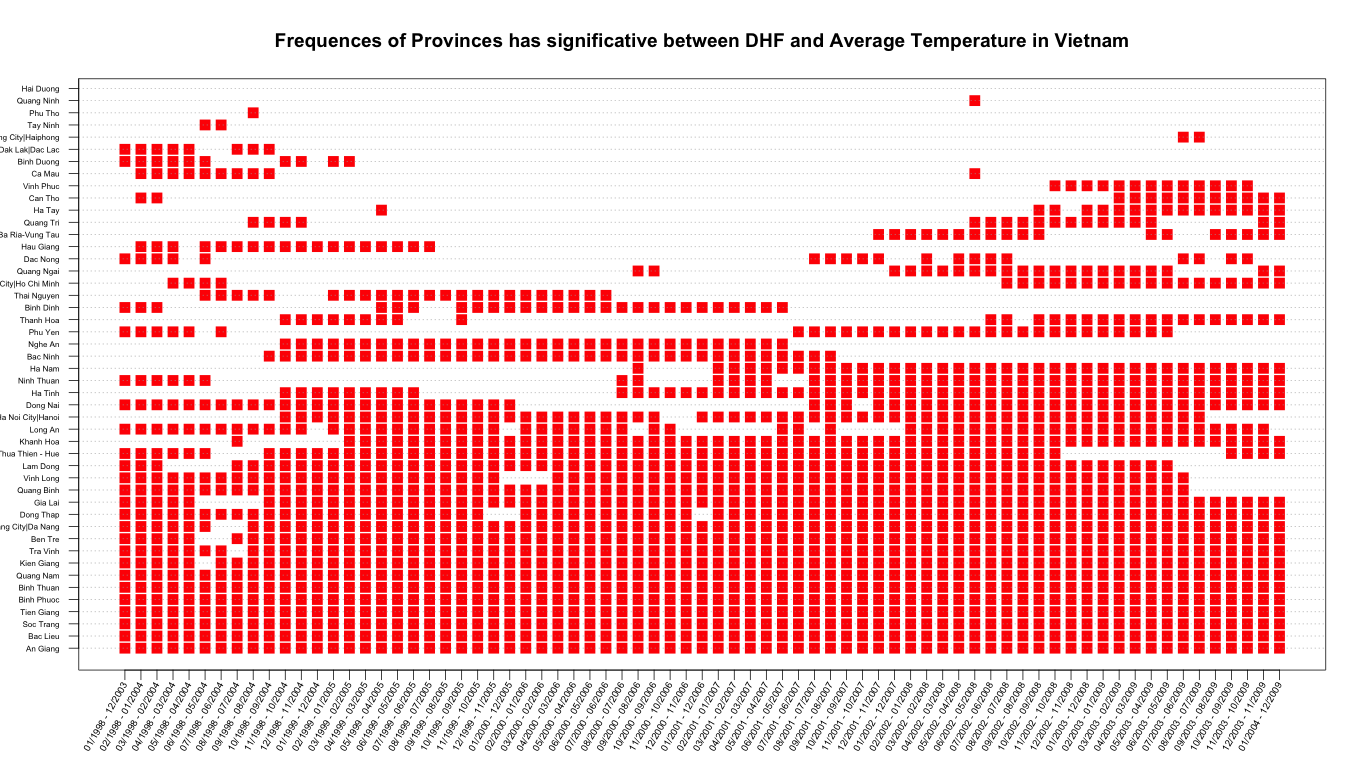
\includegraphics[width = \linewidth]{../figures/annexe/result_ta.png}
\caption{The exploration of result subsequence test with GC univariable method. The length of each period L = 6 years. The red square in each period present the relationship between dengue incidence and average temperature in this province. The Y axis is sorted by the total number of significant for every provinces over the period. }
\label{expl_1}	
\end{center}
\end{figure}

\begin{figure}[h]
\begin{center}
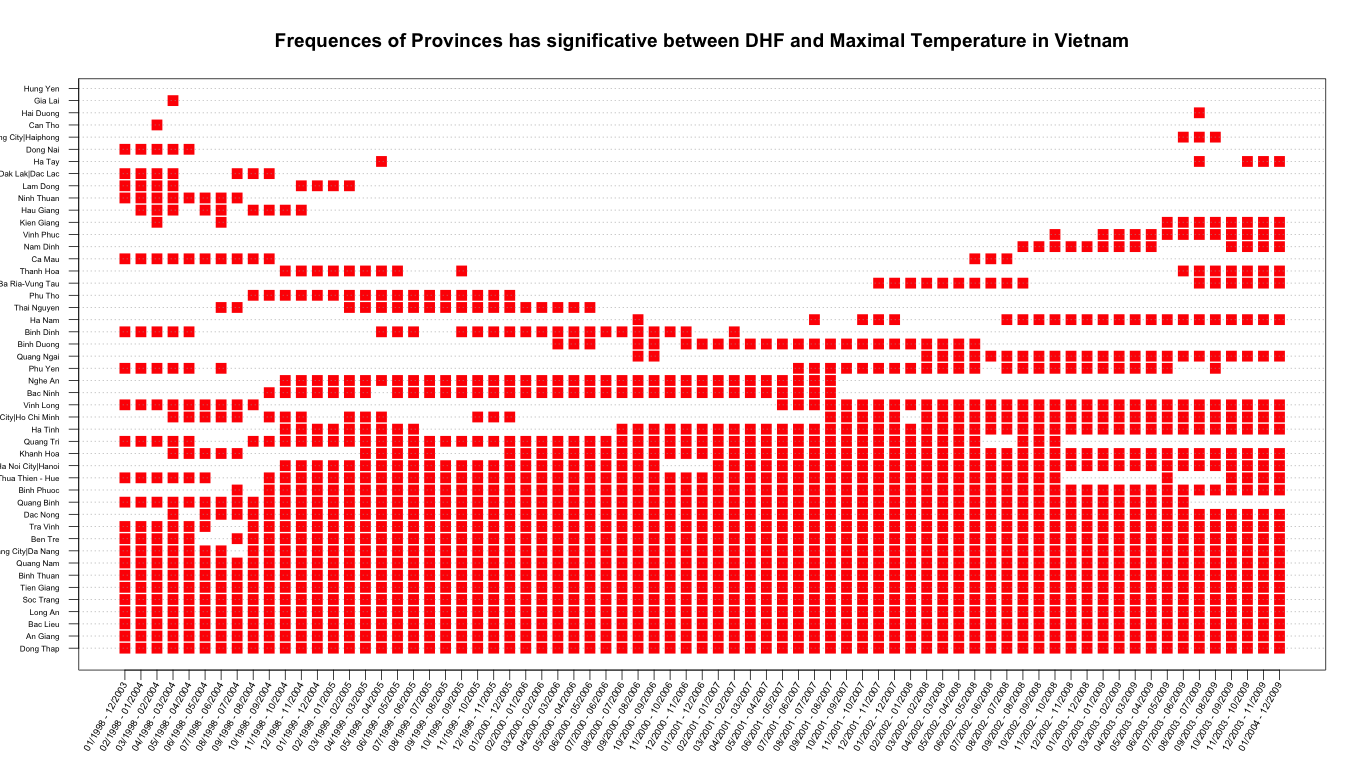
\includegraphics[width = \linewidth]{../figures/annexe/result_tx.png}
\caption{The exploration of result subsequence test with GC univariable method. The length of each period L = 6 years. The red square in each period present the relationship between dengue incidence and maximal temperature in this province. The Y axis is sorted by the total number of significant for every provinces over the period. }
\label{expl_2}	
\end{center}
\end{figure}

\begin{figure}[h]
\begin{center}
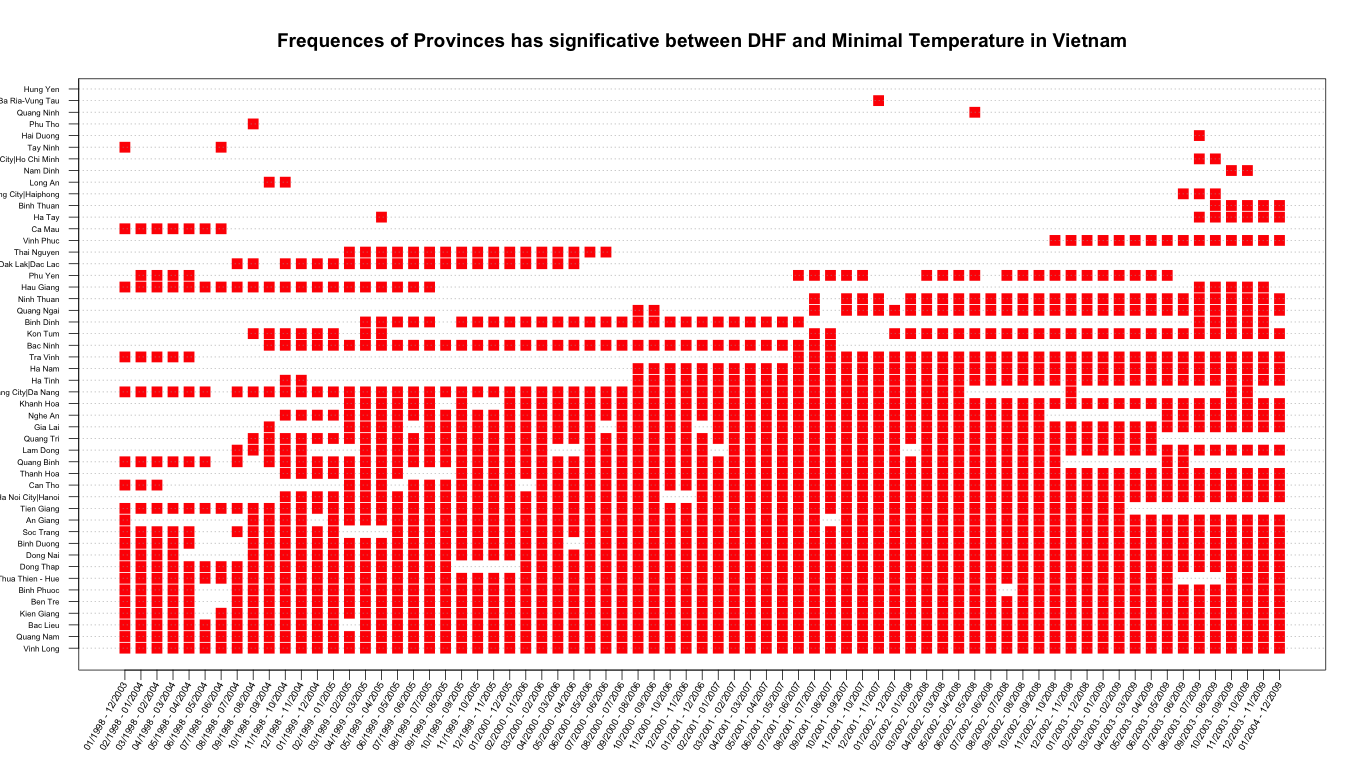
\includegraphics[width = \linewidth]{../figures/annexe/result_tm.png}
\caption{The exploration of result subsequence test with GC univariable method. The length of each period L = 6 years. The red square in each period present the relationship between dengue incidence and minimal temperature in this province. The Y axis is sorted by the total number of significant for every provinces over the period. }
\label{expl_3}	
\end{center}
\end{figure}

\begin{figure}[h]
\begin{center}
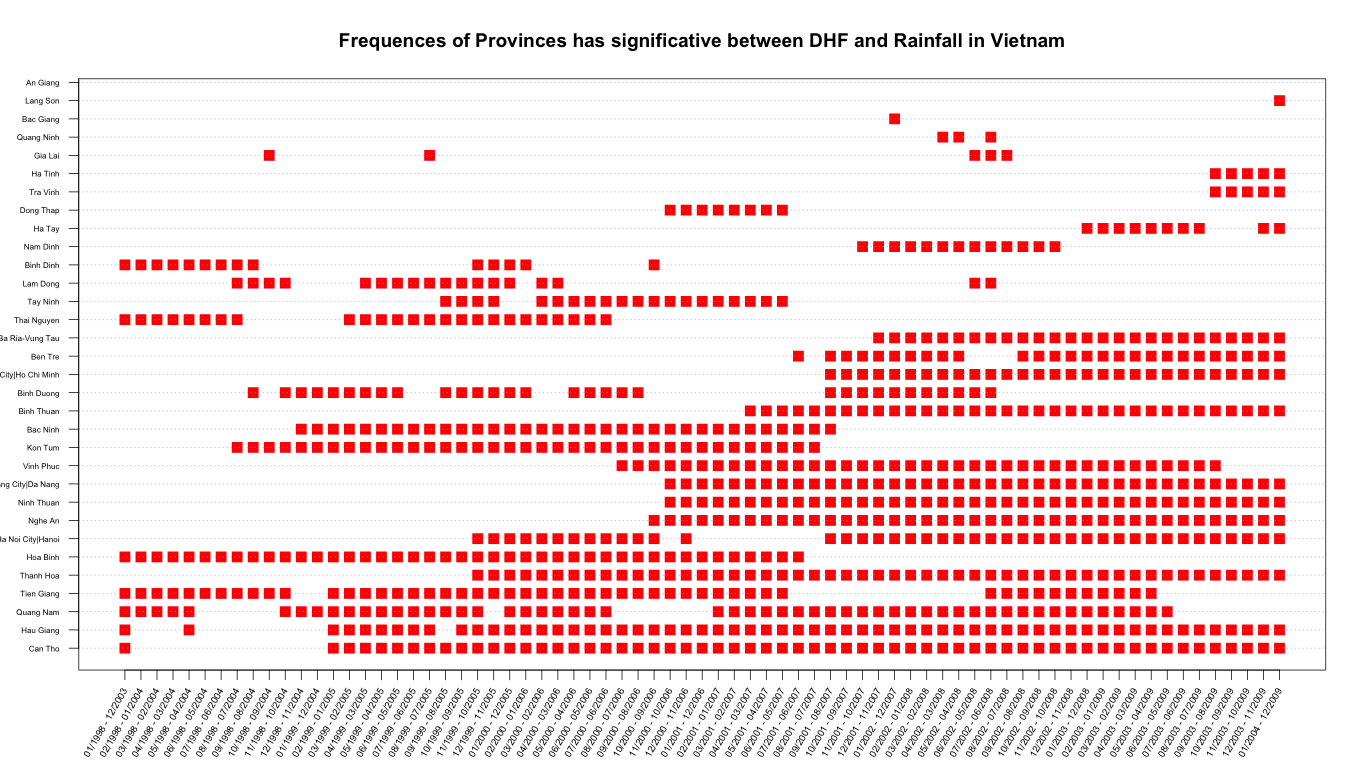
\includegraphics[width = \linewidth]{../figures/annexe/result_rf.png}
\caption{The exploration of result subsequence test with GC univariable method. The length of each period L = 6 years. The red square in each period present the relationship between dengue incidence and rainfall in this province. The Y axis is sorted by the total number of significant for every provinces over the period. }
\label{expl_4}	
\end{center}
\end{figure}

\begin{figure}[h]
\begin{center}
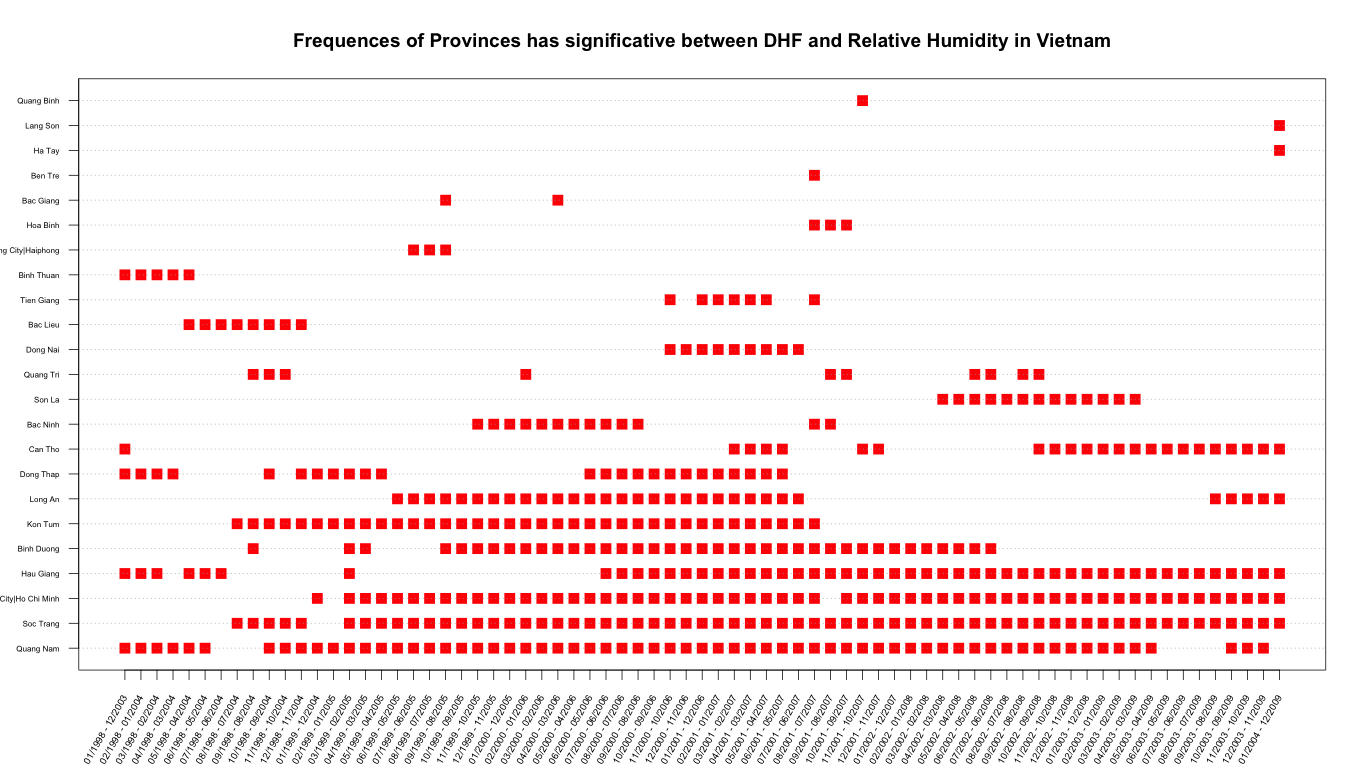
\includegraphics[width = \linewidth]{../figures/annexe/result_rh.png}
\caption{The exploration of result subsequence test with GC univariable method. The length of each period L = 6 years. The red square in each period present the relationship between dengue incidence and relative humidity in this province. The Y axis is sorted by the total number of significant for every provinces over the period. }
\label{expl_5}	
\end{center}
\end{figure}

\begin{figure}[h]
\begin{center}
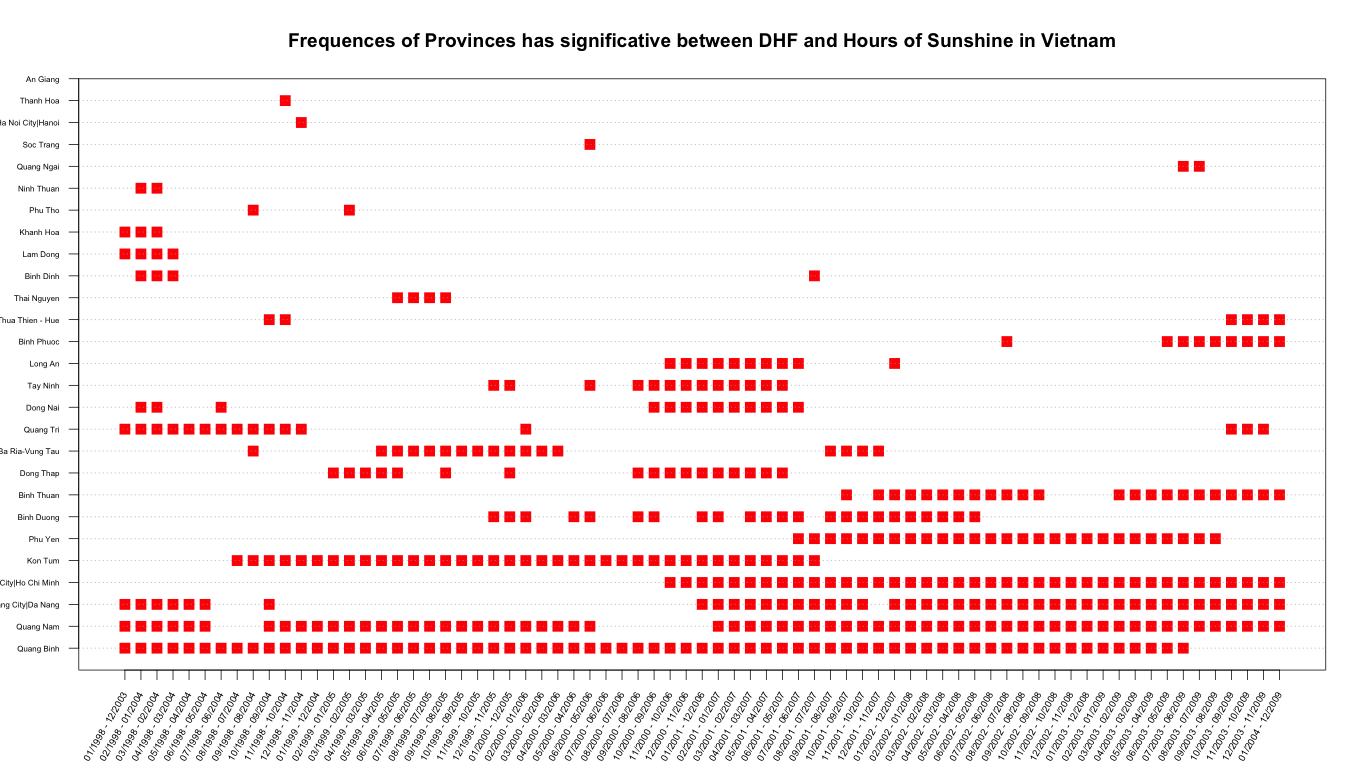
\includegraphics[width = \linewidth]{../figures/annexe/result_sh.png}
\caption{The exploration of result subsequence test with GC univariable method. The length of each period L = 6 years. The red square in each period present the relationship between dengue incidence and hours of sunshine in this province. The Y axis is sorted by the total number of significant for every provinces over the period. }
\label{expl_6}	
\end{center}
\end{figure}

\begin{figure}[h]
\begin{center}
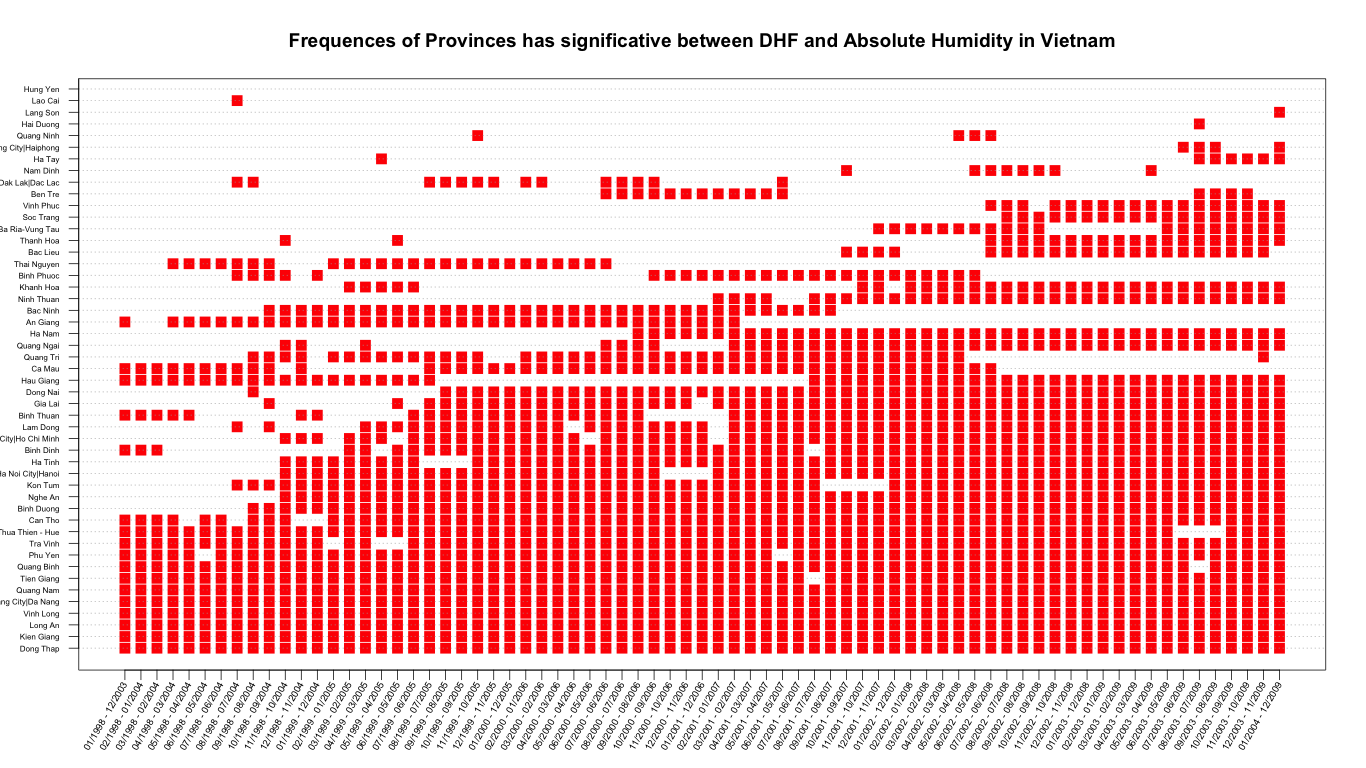
\includegraphics[width = \linewidth]{../figures/annexe/result_ah.png}
\caption{The exploration of result subsequence test with GC univariable method. The length of each period L = 6 years. The red square in each period present the relationship between dengue incidence and absolute humidity in this province. The Y axis is sorted by the total number of significant for every provinces over the period. }
\label{expl_7}	
\end{center}
\end{figure}

%%%%%%%
% clasified by lattitude


\begin{figure}[h]
\begin{center}
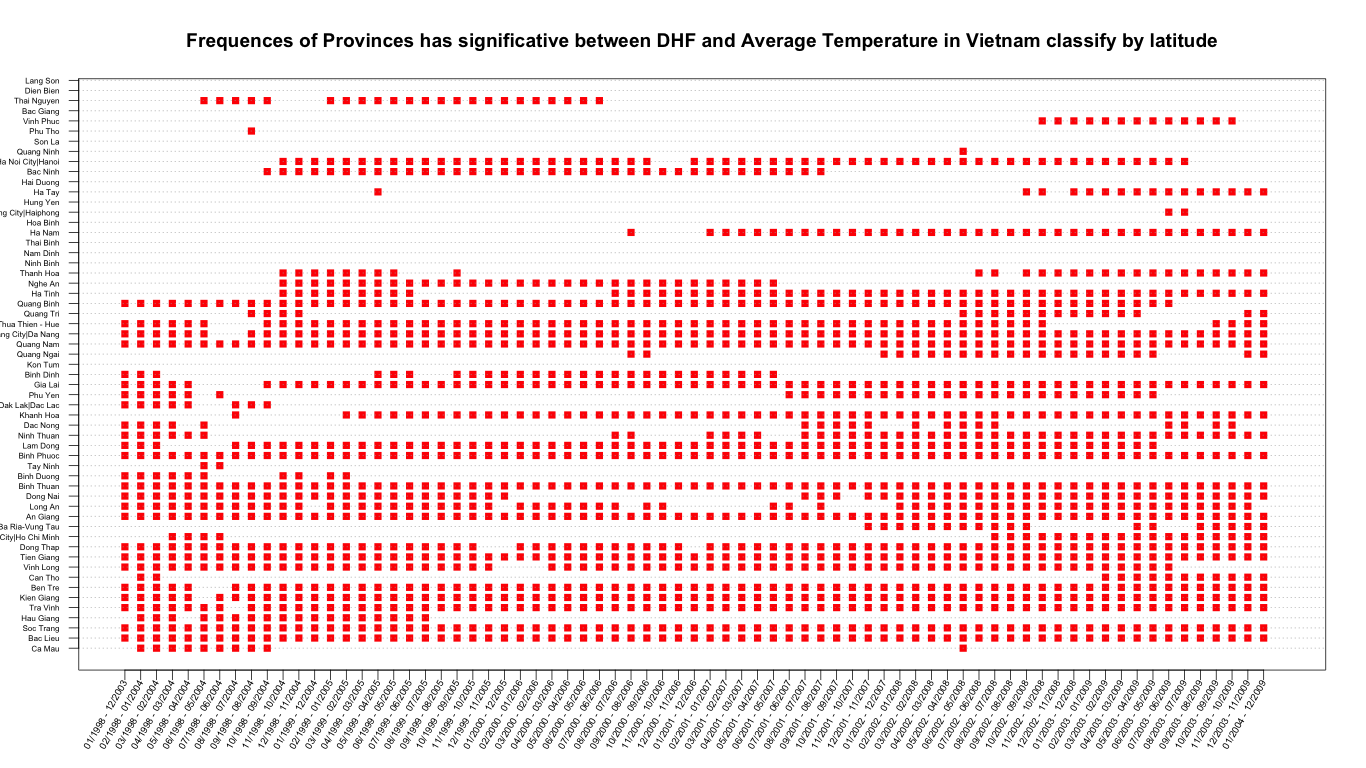
\includegraphics[width = \linewidth]{../figures/annexe/lat_result_ta.png}
\caption{The exploration of result subsequence test with GC univariable method. The length of each period L = 6 years. The red square in each period present the relationship between dengue incidence and average temperature in this province. Provinces on Y axis are ordered according to their latitude.  }
\label{expl_8}	
\end{center}
\end{figure}

\begin{figure}[h]
\begin{center}
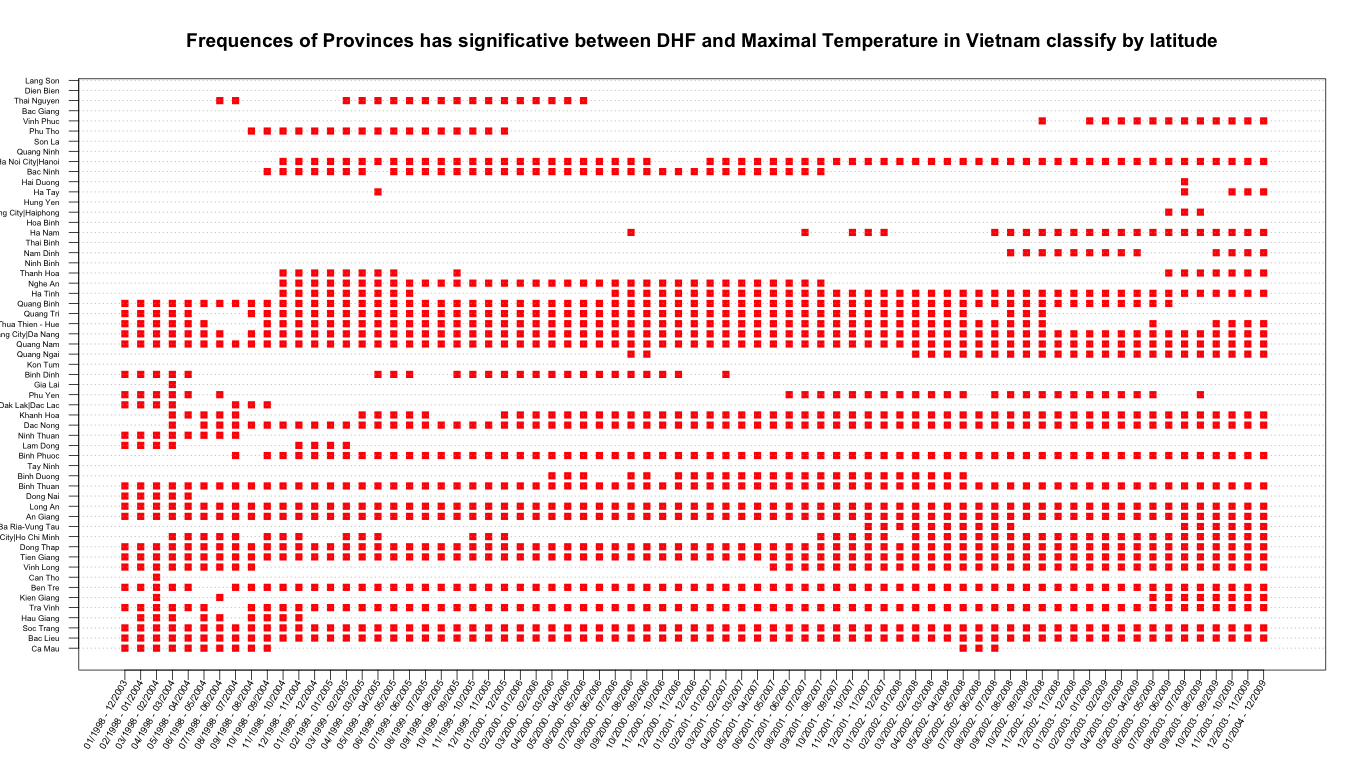
\includegraphics[width = \linewidth]{../figures/annexe/lat_result_tx.png}
\caption{The exploration of result subsequence test with GC univariable method. The length of each period L = 6 years. The red square in each period present the relationship between dengue incidence and maximal temperature in this province. Provinces on Y axis are ordered according to their latitude.  }
\label{expl_9}	
\end{center}
\end{figure}

\begin{figure}[h]
\begin{center}
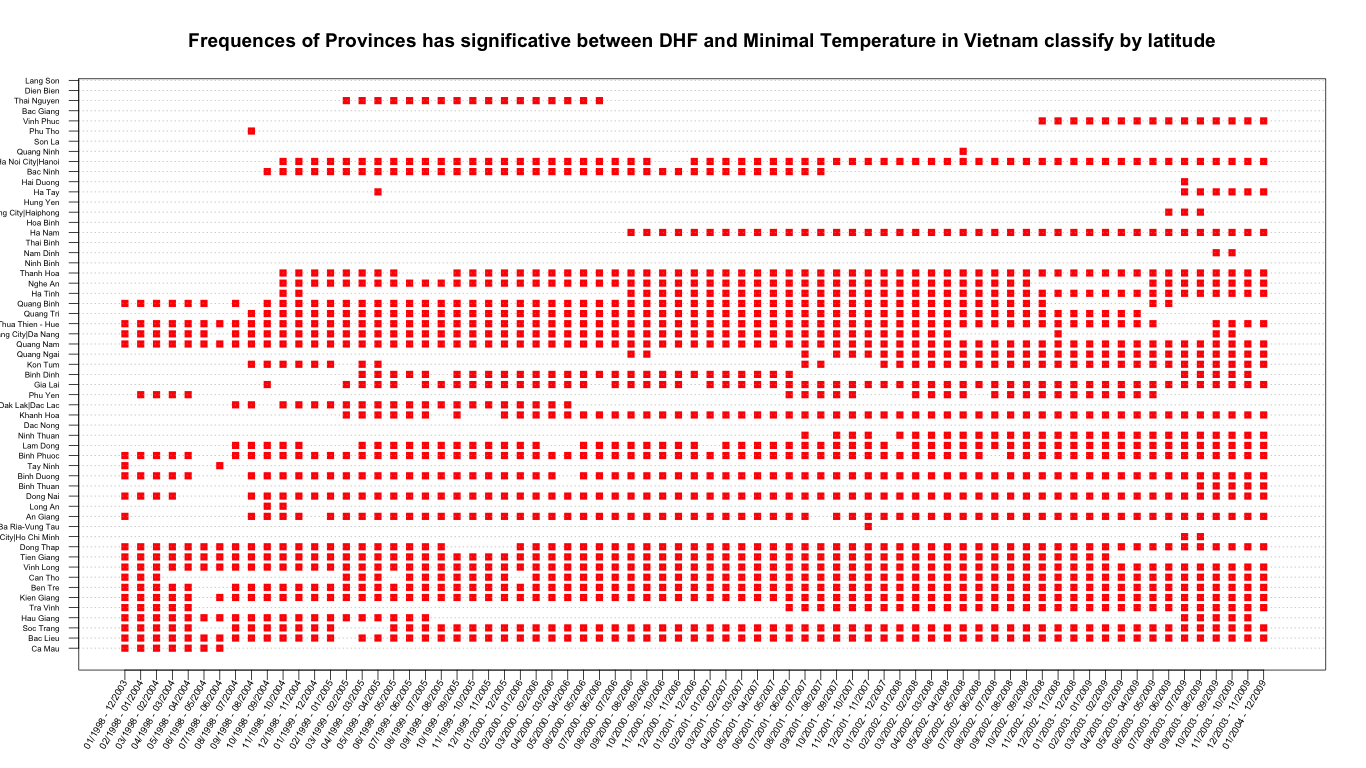
\includegraphics[width = \linewidth]{../figures/annexe/lat_result_tm.png}
\caption{The exploration of result subsequence test with GC univariable method. The length of each period L = 6 years. The red square in each period present the relationship between dengue incidence and minimal temperature in this province. Provinces on Y axis are ordered according to their latitude.  }
\label{expl_10}	
\end{center}
\end{figure}

\begin{figure}[h]
\begin{center}
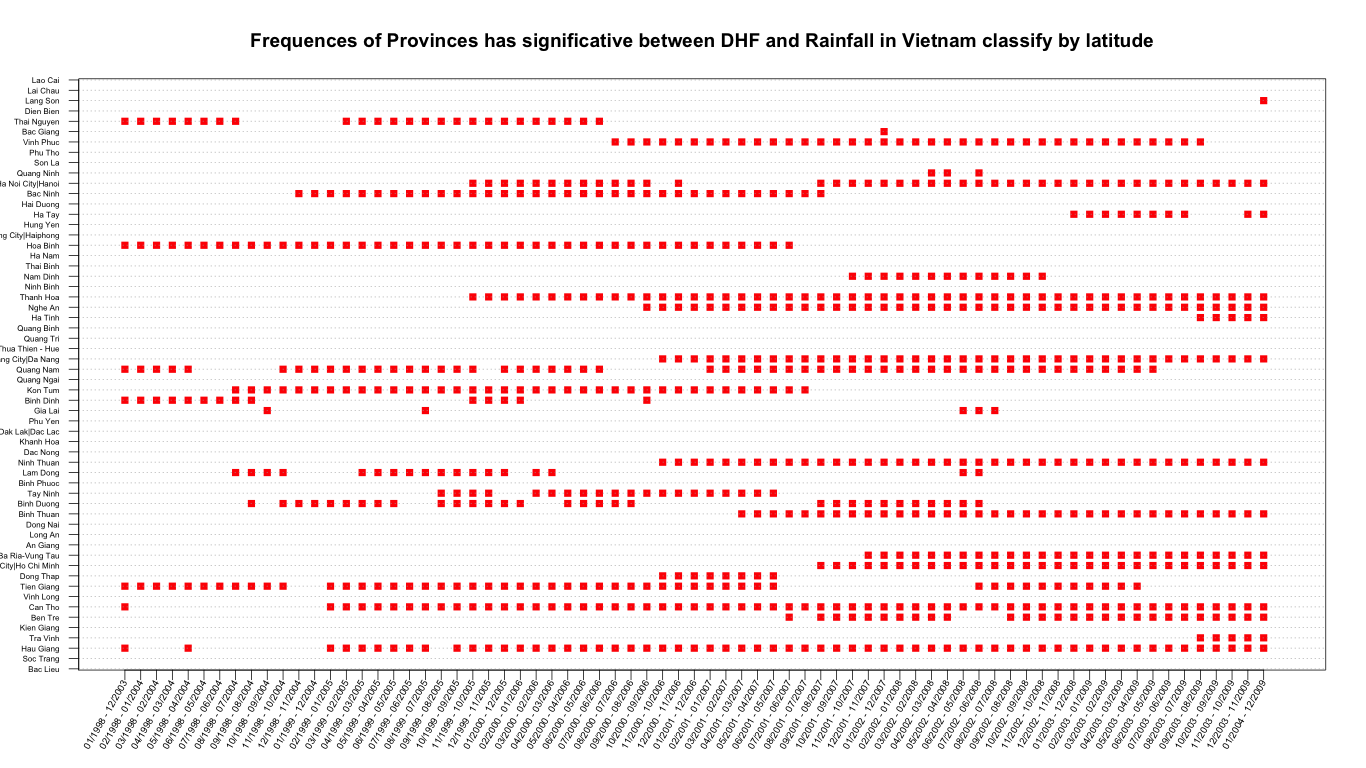
\includegraphics[width = \linewidth]{../figures/annexe/lat_result_rf.png}
\caption{The exploration of result subsequence test with GC univariable method. The length of each period L = 6 years. The red square in each period present the relationship between dengue incidence and rainfall in this province. Provinces on Y axis are ordered according to their latitude.  }
\label{expl_11}	
\end{center}
\end{figure}

\begin{figure}[h]
\begin{center}
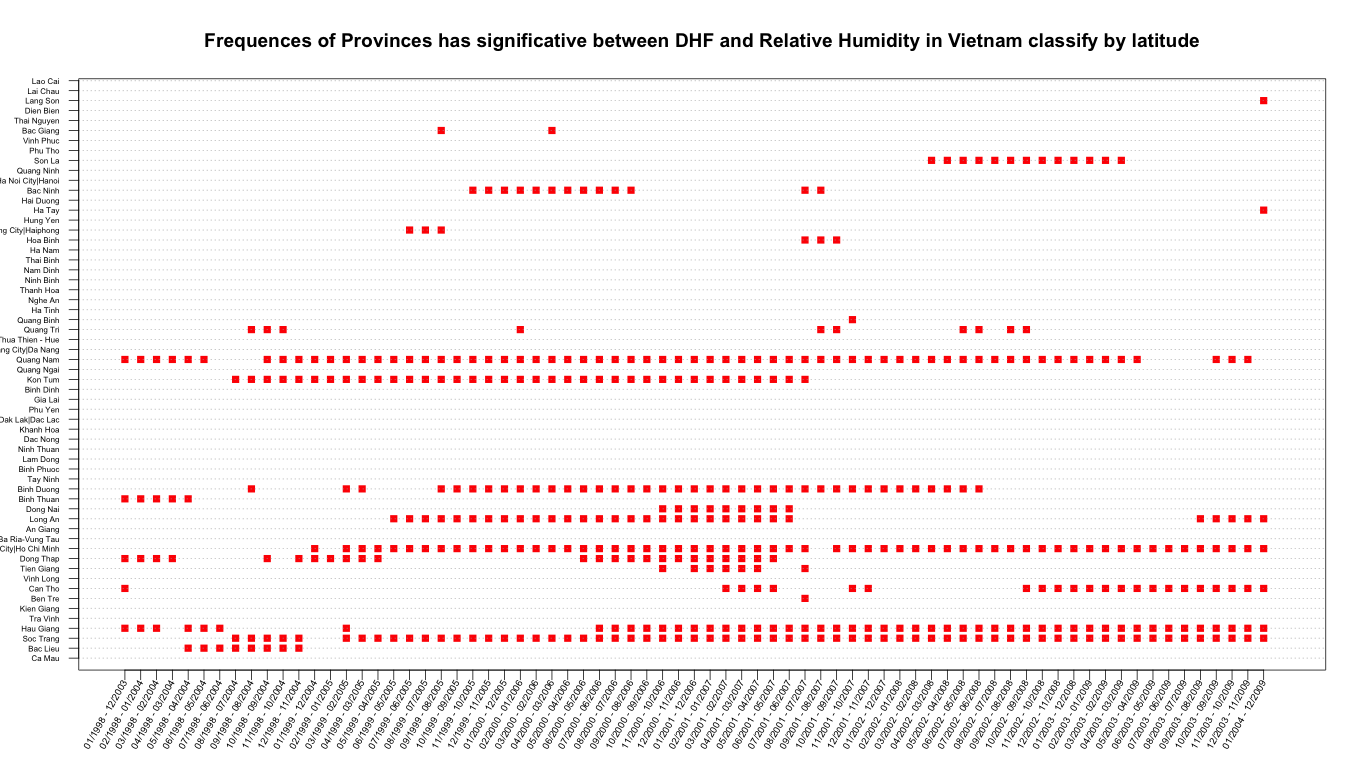
\includegraphics[width = \linewidth]{../figures/annexe/lat_result_rh.png}
\caption{The exploration of result subsequence test with GC univariable method. The length of each period L = 6 years. The red square in each period present the relationship between dengue incidence and relative humidity in this province. Provinces on Y axis are ordered according to their latitude. }
\label{expl_12}	
\end{center}
\end{figure}

\begin{figure}[h]
\begin{center}
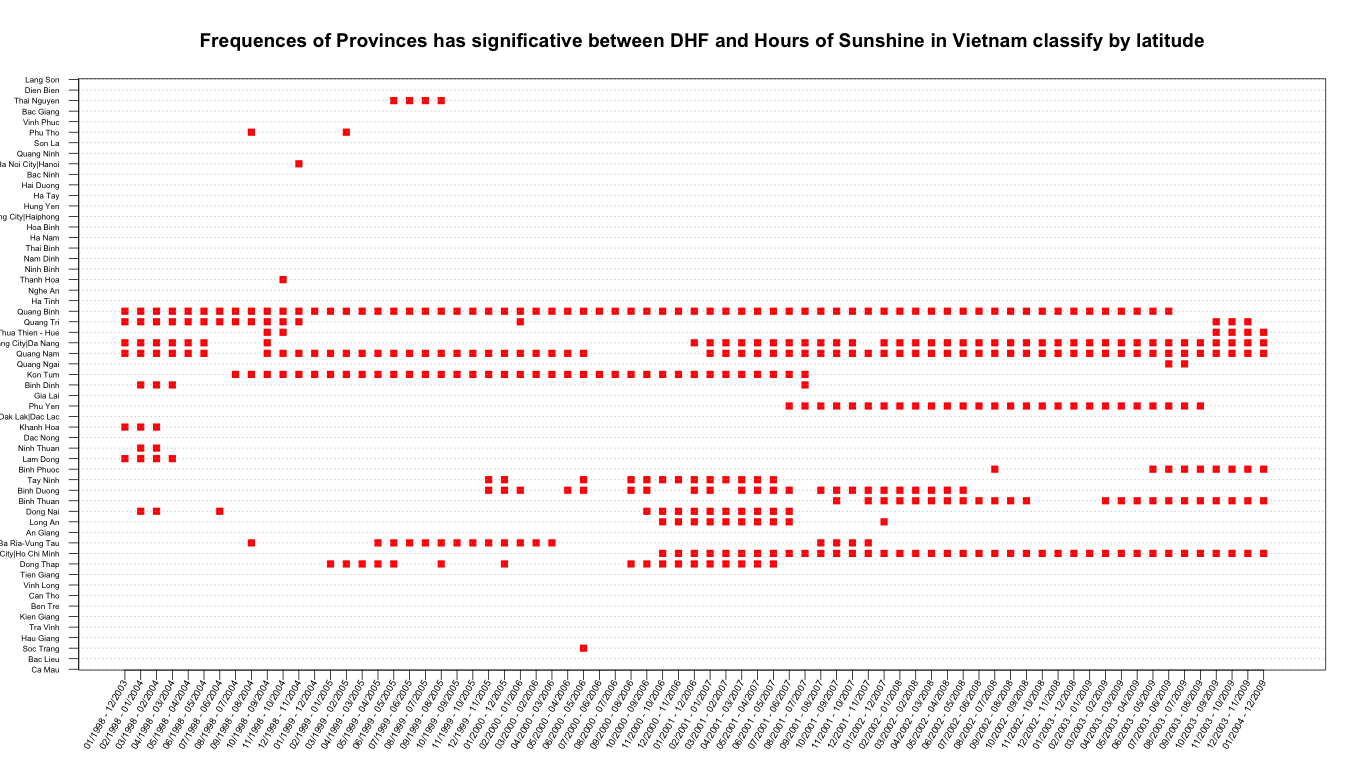
\includegraphics[width = \linewidth]{../figures/annexe/lat_result_sh.png}
\caption{The exploration of result subsequence test with GC univariable method. The length of each period L = 6 years. The red square in each period present the relationship between dengue incidence and hours of sunshine in this province. Provinces on Y axis are ordered according to their latitude. . }
\label{expl_13}	
\end{center}
\end{figure}

\begin{figure}[h]
\begin{center}
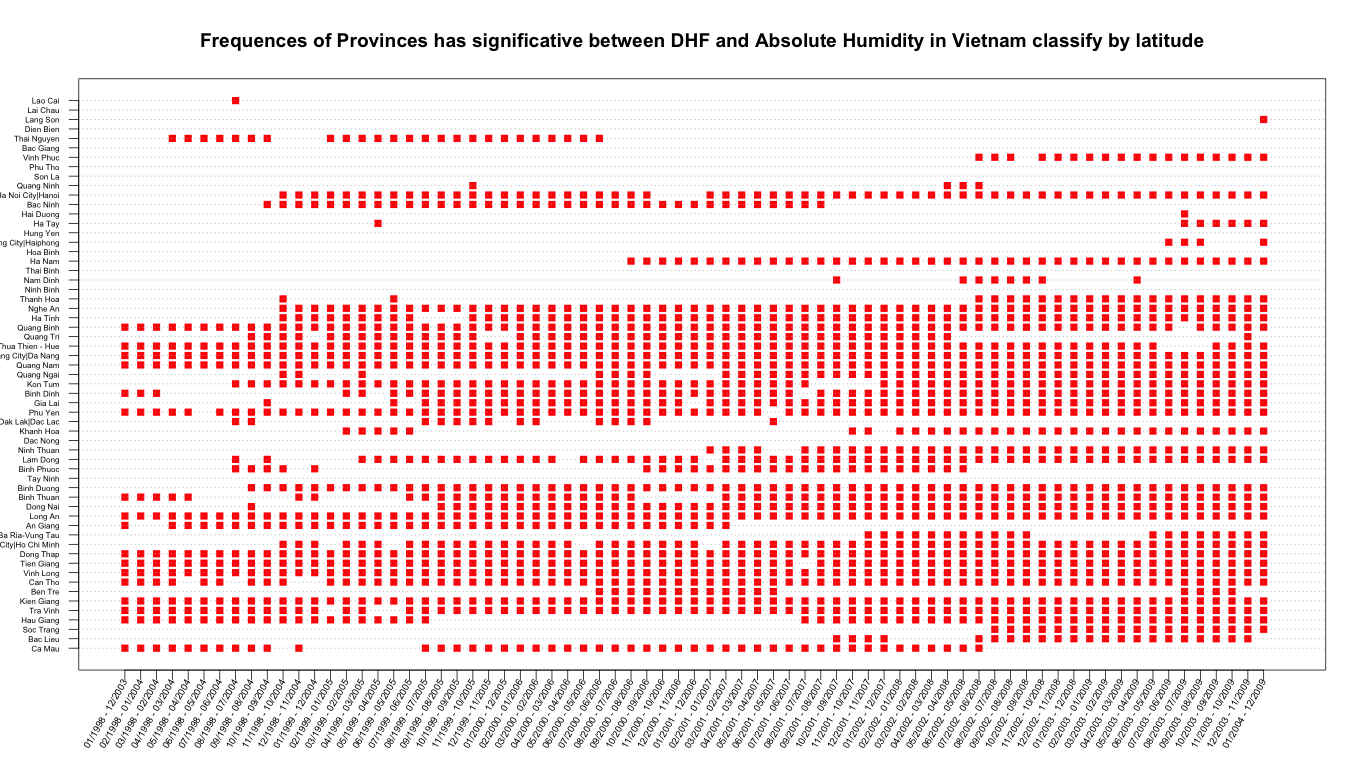
\includegraphics[width = \linewidth]{../figures/annexe/lat_result_ah.png}
\caption{The exploration of result subsequence test with GC univariable method. The length of each period L = 6 years. The red square in each period present the relationship between dengue incidence and absolute humidity in this province. Provinces on Y axis are ordered according to their latitude. }
\label{expl_14}	
\end{center}
\end{figure}

